\documentclass[../ut-dissertation.tex]{subfiles}
\begin{document}

\chapter{Results}
This chapter contains the results of two sample runs of the model.
The first is a simple example which is intended to show what the
model's results look like.  The second example is the result of the
classification of a regional conference paper.

\section{A Simple Example}
One of the problems with a model such as this one is that ground truth
is difficult to arrive at.  In fact, this model quantifies a property
which even the author of the documents in question may be unaware of.
As such, verification of the model depends on the sensibility of its
answers.  However, this again presents a challenge because the total
structure of the all of the factors and relationships among them is
very complex and difficult to visualize.  To help alleviate this
problem, this section contains a very simple example, one in which all
of the components of the model may be seen.  This example uses three
simple stories, written for this purpose, drawing on a 30 word
vocabulary.  The first story is in Figure~\ref{fig:cat_story}, the
second is in Figure~\ref{fig:dog_story}, and the third is in
Figure~\ref{fig:cat_dog_story}.  The third story is intended to be a
sequel of sorts, drawing on material from the previous stories.  The
complete vocabulary for this example is shown in
Table~\ref{tab:catdog_vocabulary}.
\begin{figure}
  \noindent\fbox{%
    \parbox{\textwidth}{%
     The cat sat on the mat.  The cat was happy to be on the mat.  The cat
     saw the mouse running but was too lazy to chase it.
   }}
  \caption{The Cat's Tale}\label{fig:cat_story}
\end{figure}

\begin{figure}
  \noindent\fbox{%
    \parbox{\textwidth}{%

    The dog walked to the house.  The dog saw the food bowl, and the
    dog saw a squirrel.  The dog chased the squirrel from the food
    bowl.
  }}
  \caption{The Dog's Tale}\label{fig:dog_story}
\end{figure}

\begin{figure}
  \noindent\fbox{%
    \parbox{\textwidth}{%
    The dog saw the cat on the mat.  The dog walked to the house, and
    the dog chased the cat.  The squirrel was happy to see the dog
    chase the cat on the mat.  The dog saw the squirrel, and decided
    to chase the squirrel instead.  The cat sat on the mat.
}}
  \caption{The Saga Continues}\label{fig:cat_dog_story}
\end{figure}

\begin{table}
  \centering
  \begin{tabular}{c|l||c|l}
    $I$ & Word & $I$ & Word\\ 
    \hline
    1 & the & 16 & chased \\
    2 & house & 17 & sat \\
    3 & mouse & 18 & be \\
    4 & squirrel & 19 & happy \\
    5 & it & 20 & on\\
    6 & saw & 21 & from \\
    7 & lazy & 22 & food \\
    8 & cat & 23 & decided \\
    9 & mat & 24 & to\\
   10 & a & 25 & was \\
   11 & bowl & 26 & dog \\
   12 & walked & 27 & running \\
   13 & too & 28 & instead \\
   14 & and & 29 & but \\
   15 & see & 30 & chase\\
  \end{tabular}
  \caption{Cat and Dog Vocabulary}\label{tab:catdog_vocabulary}
\end{table}

After a few trial decompositions, 7 factors was determined to be the
optimal decomposition of the document corpus.  This yielded an error
ratio of 0.45, which is the best fit can yield.  (The range of values
tried was from 1 to the number of non-zero elements in the tensor.)
Even with this relatively poor fit, the model was able to distinguish
features of the stories.  The distances between the factors, other
than the diagonals, range from 0 to 1.4.  The final classification
step yielded the classification of factors shown in
Table~\ref{tab:cat_dog_class}.

The model threshold value as set to 0.2, which is a sensible value as
this requires a 90\% match in a factor.  In this case it would not
have mattered, however, as the matching factors were all perfect
matches with an $L_1$ distance of 0.

\begin{table}
  \centering
  \begin{tabular}{|l|c|l|}
    \hline
    Factor & Factor Weight & Classification\\
    \hline
    1 & 0.28 & Author Contribution\\
    \hline
    2 & 0.15 & Cat Factor 1\\
    \hline
    3 & 0.14 & Author Contribution\\
    \hline
    4 & 0.14 & Author Contribution\\
    \hline
    5 & 0.11 & Author Contribution\\
    \hline
    6 & 0.11 & Author Contribution\\
    \hline
    7 & 0.06 & Dog Factor 1\\
    \hline
  \end{tabular}
  \caption{Cat Dog Model} \label{tab:cat_dog_class}
\end{table}

The final classification of the contribution of the 3 sources, the cat
story, the dog story, and the author's original contributions are
shown in Figure~\cite{fig:cat_dog_bar}.

\begin{figure}
  \centering
  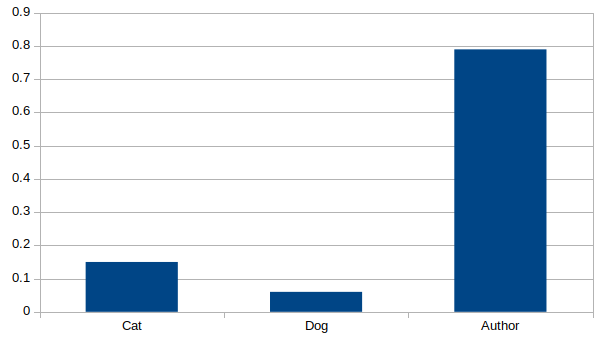
\includegraphics[width=3.5in]{diagrams/catdog}
  \caption{Cat Dog Saga Contributions}
\end{figure}

The factors discovered by this process are as follows.  Factor 1, with
its non-zero entries translated into the words they represent contains
most of the situational and action oriented parts of the sequel.
\begin{itemize}
\item saw the squirrel 0.267417
\item saw the cat 0.223651
\item saw the dog 0.192194
\item cat the squirrel 0.044066
\item cat the cat 0.036854
\item cat the dog 0.031670
\item mat the squirrel 0.034331
\item mat the cat 0.028712
\item mat the dog 0.024674
\item see the squirrel 0.032132
\item see the cat 0.026873
\item see the dog 0.023094
\item chased the squirrel 0.013437
\item chased the cat 0.011238
\item chased the dog 0.009657
\end{itemize}

The second factor, which was matched to the cat story consists of just
one phrase, which aptly describes the cat's outlook on life.
\begin{itemize}
\item on the mat 1.000000
\end{itemize}

The third factor deals mainly with the squirrel.  Note that the
decomposition process actually invented a phrase which does not appear
in the story.  This is due to the small amount of data, and therefore
smaller chance of fitting factors to the model.
\begin{itemize}
\item squirrel and happy 0.249836
\item squirrel and decided 0.262960
\item squirrel was happy 0.237368
\item squirrel was decided 0.249836
\end{itemize}

The fourth factor contains the dog's primary thought process.  Note
that the dog only makes decisions in the sequel.
\begin{itemize}
\item decided to chase 1.000000
\end{itemize}

The fifth factor contains a response from the cat which only appears
in the sequel.
\begin{itemize}
\item happy to see 1.000000
\end{itemize}

The sixth factor contains the action found in the sequel.
\begin{itemize}
\item cat saw the 0.345830
\item cat see the 0.040819
\item cat chased the 0.172914
\item cat chase the 0.213734
\item walked saw the 0.056987
\item walked see the 0.006726
\item walked chased the 0.028493
\item walked chase the 0.035220
\item to saw the 0.044398
\item to see the 0.005240
\item to chased the 0.022199
\item to chase the 0.027439
\end{itemize}

Finally, the seventh factor gives us all the actions that the dog
carries out.  This one was matched to the dog's story, which is where
we first learn the things the dog likes to do!
\begin{itemize}
\item  the dog saw 0.400000
\item the dog walked 0.200000
\item the dog chased 0.200000
\item the dog chase 0.200000
\end{itemize}

The separation that the model accomplished, even with very scant data,
shows that the expected similarities in the resultant factors are
present.  The next step is to look at a more substantial example.


\section{A Conference Paper Case Study}
For a real-world case study, a conference paper was pulled from the
ACM Digital library.  This was the first paper listed in the first
conference listed in their regional conference proceedings.  This
paper cites four other papers and two websites.  The two websites were
used to pull data, and so they are not included in the corpus.  In
addition to the four cited papers, two unrelated papers are included
to test if the model will select factors from these unrelated papers.
The complete corpus, listed with the target paper last, is shown in
Table~\ref{tab:conference_corpus}. Documents 1-4 are the papers cited
by the target paper, documents 5-6 are unrelated papers, and document
7 is the target paper.

\begin{table}
  \centering
  \begin{tabular}{|l|l|}
    \hline
    1 & Jessica Lin, Eamonn Keogh, Stefano Lonardi, and Bill Chiu. A\\
      & symbolic representation of time series, with implications for\\
      & streaming algorithms. In Proc. DMKD 2003, pages 2–11. ACM
        Press, 2003.\\
    \hline
    2 & Andreas Schlapbach and Horst Bunke. Using hmm\\
      & based recognizers for writer identification and\\
      & verification. In Proc. FHR 2004, pages 167–172. IEEE, 2004.\\
    \hline
    3 & Yusuke Manabe and Basabi Chakraborty. Identity\\
      & detection from on-line handwriting time series. In Proc.\\
      & SMCia 2008, pages 365–370. IEEE, 2008.\\
    \hline
    4 & Sami Gazzah and Najoua Ben Amara. Arabic \\
      & handwriting texture analysis for writer identification\\
      & using the dwt-lifting scheme. In Proc. ICDAR 2007,\\
      & pages 1133–1137. IEEE, 2007.\\
    \hline
    5 & Kolda, Tamara Gibson. Multilinear operators for higher-order \\
      & decompositions. 2006\\
    \hline
    6 & Blei, David M and Ng, Andrew Y and Jordan, Michael I. Latent\\
      & dirichlet allocation. 2007\\
    \hline
    \hline
    7 & Serfas, Doug. Dynamic Biometric Recognition of Handwritten Digits\\
      & Using Symbolic Aggregate Approximation. Proceedings of the ACM\\
      & Southeast Conference 2017\\
    \hline
  \end{tabular}
  \caption{Conference Paper Corpus}\label{tab:conference_corpus}
\end{table}

The entire corpus consists of 45,152 words.  As described in the
previous chapter, the vocabulary was truncated to 600 words.  The 600
words were the most frequent words across the corpus.  The other
parameters are shown in Table~\ref{tab:model_parameters}
\begin{table}
  \centering
  \begin{tabular}{ccc}
    \hline
    $n$ & $nfactors$ & $threshold$\\
    \hline
    3 & 150 & 0.2\\
    \hline
  \end{tabular}
  \caption{Conference Model Parameters}\label{tab:model_parameters}
\end{table}
\end{document}
Again, 0.2 is used as the threshold as it is a good default setting.
The decomposition of the 7 documents into 150 factors was carried out
on a machine with a 3.9GHz 8-core Intel processor and 15GB of RAM.
The decomposition and construction of normalized tensors took
approximately 2.5 hours to complete. Calculation of the distance
matrix and classifying the factors required another hour and a half.
The results are shown in Table~\ref{tab:conference_results}.


\begin{table}
  \centering
  \begin{tabular}{l|c|l|}
    \hline
    Document & Influence & Number of Matched Factors\\
    \hline
    1 & 0.21 & 10\\
    2 & 0.09 & 9\\
    3 & 0.06 & 3\\
    4 & 0.06 & 1\\
    5 & 0.00 & 0\\
    6 & 0.00 & 0\\
    Author & 0.57 & 127\\
  \end{tabular}
  \caption{Conference Classification Results}\label{tab:conference_results}
\end{table}

As these results show, the model makes a set of reasonable matches,
and it does not select unrelated documents.  The actual makeup of the
factors are much more complex, however ideas can be traced through
them.  Unfortunately, these factors are much too large to be included
verbatim in this chapter. However, the factors that were matched from
paper one all deal with a technique which generates a symbolic
representation of a time series.  This technique serves as the basis
for the invention in the paper, and is talked about many times with
many of the same explanations used in the first paper.  Thus the model
has not only avoided unrelated information, it has given a greater
weight to the paper which had the greatest semantic influence on the
work being studied.
